\chapter{Hive Query}

	Query to find the max, min, total, average stay per user per country by using only Hive Query turned out to be inefficient. This is because we need to use triple join, which will be highly inefficient for big data queries. 
	
	To avoid this we have used Hive Query and a map reduce job to achieve our objective
		
\section{Design}
	So we split the task into three parts \\
	\begin{itemize}
		\item [Part1:] Join Place Table and Photos Table to produce table containing \(Owner, Date Taken, Country\). \\
		We have use Hive Query for this job because writing query for this task is simple as a SQL Query. This makes code readable for everyone. 
		\item [Part2:] Map Job to return the content as it is but distribute by Owner and Sort it by date. 
		For distributing and sorting we have leveraged Map reduce framework.
		\item [Part3:] Reduce Job to Find the Max, Min, Average, Total stay per User Per Country. 
		We used python script to do the reduce as this is simple to sequentially go through the time sorted list and find out the time a user stayed in each country. 
	\end{itemize}

\section{Lineage}
	
\usetikzlibrary{shapes.geometric,arrows}

\tikzstyle{decision} = [ diamond, draw, fill=blue!20, text width=4.5em, text badly centered, node distance=3cm, inner sep-0pt]  
\tikzstyle{block} = [ rectangle, draw, fill=blue!20, text width=15em, text badly centered, rounded corners, minimum height=4em]  
\tikzstyle{line} = [ draw, -latex']  
\tikzstyle{terminator} = [ draw, ellipse, fill=red!20, node distance=3cm, minimum height=2em]  

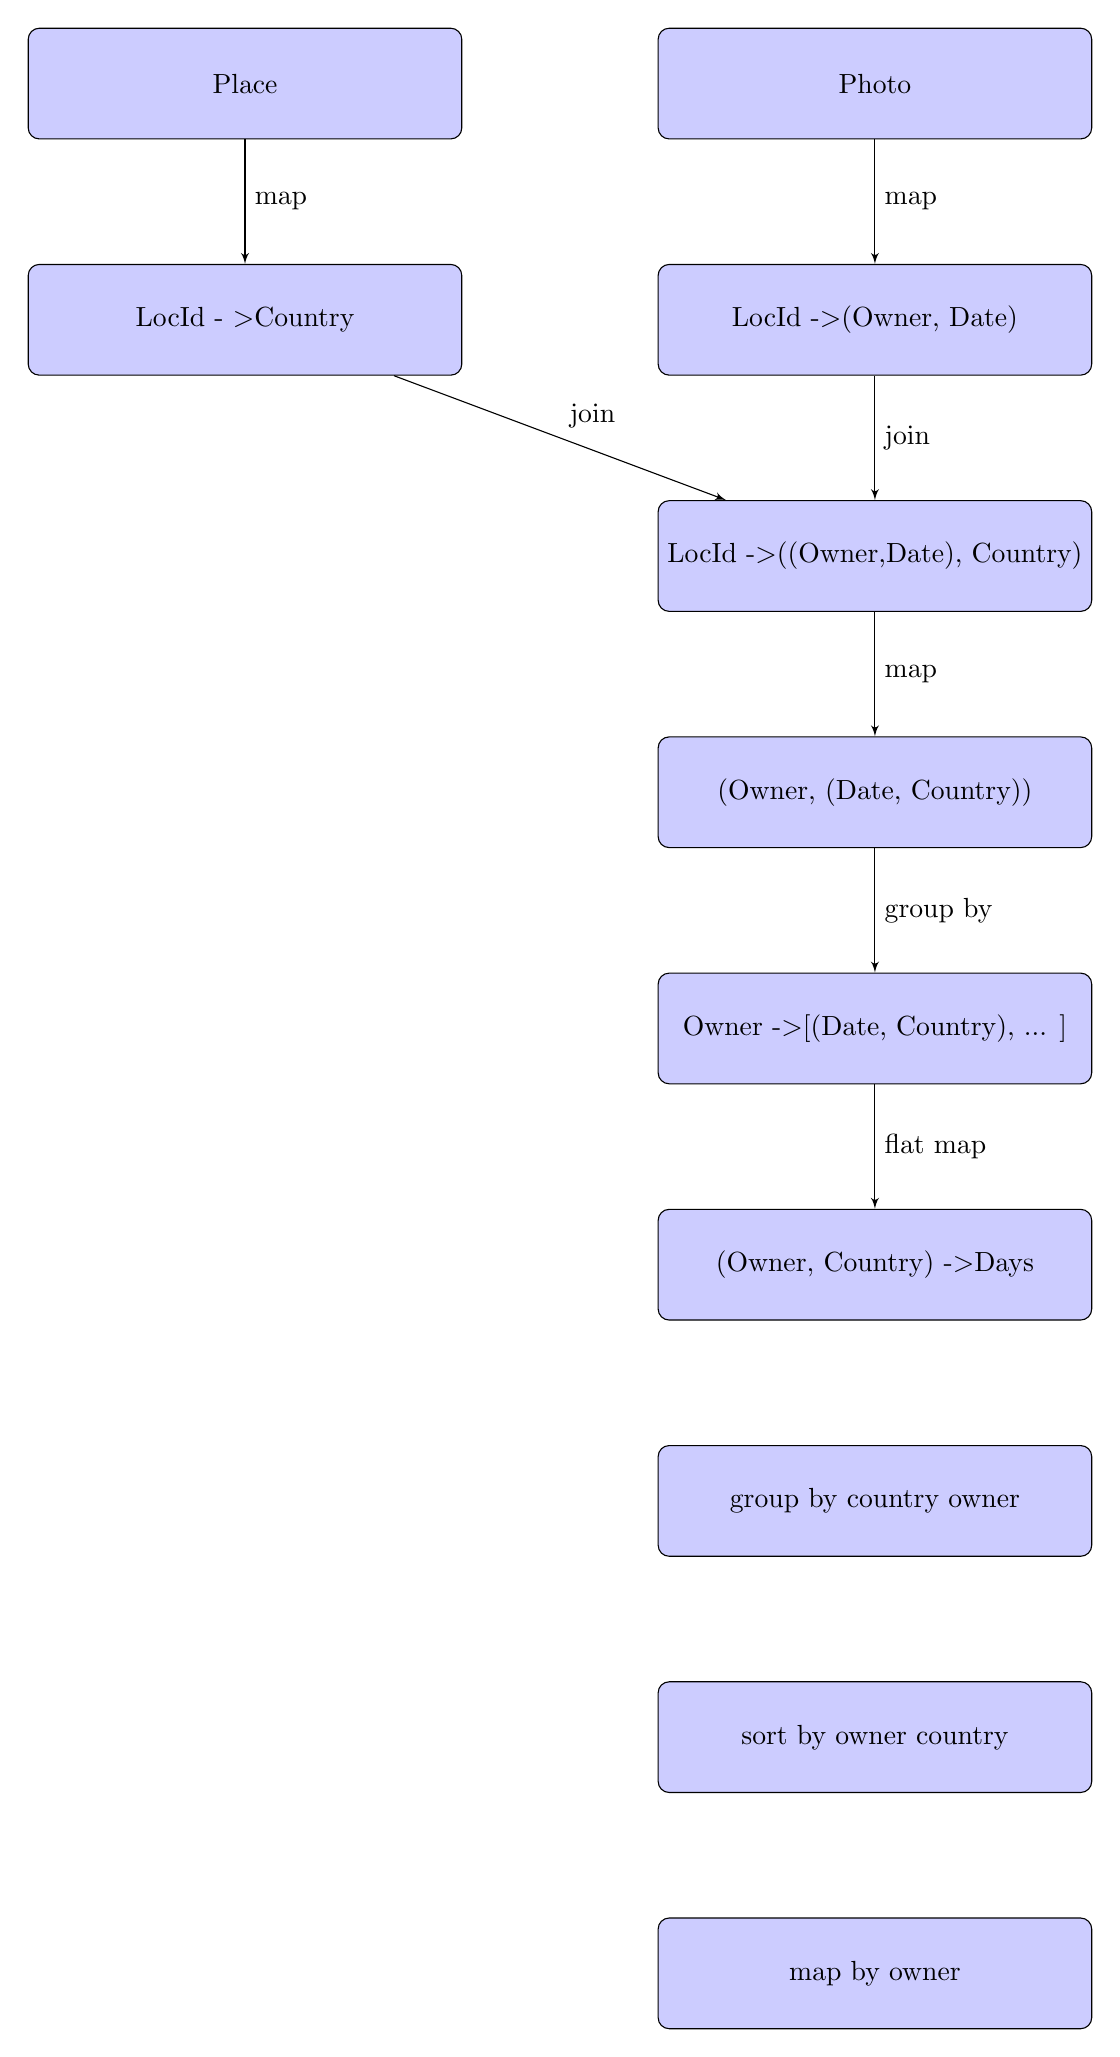
\begin{tikzpicture}[node distance=3cm, auto]   
  \node [block]  (place)  {Place};  
  \node [block, below of=place]  (place_map) {LocId - 	\textgreater Country};  
  
  \node [block, right of=place, xshift=5cm]  (photo)  {Photo};
  \node [block, below of=photo]  (photo_map) {LocId -\textgreater (Owner, Date)};  
  
  \node [block, below of=photo_map] (join) {LocId -\textgreater ((Owner,Date), Country)};
  
  \node [block, below of=join] (join_map) {(Owner, (Date, Country))};
  
  \node [block, below of=join_map] (group_by_owner) {Owner -\textgreater [(Date, Country), ... ]};
  \node [block, below of=group_by_owner] (flatmap_owner) {(Owner, Country) -\textgreater Days};
  
  \node [block, below of=flatmap_owner] (grpby_owner_country) {group by country owner};
  
  \node [block, below of=grpby_owner_country] (sort_by_owner_country) {sort by owner country};
  \node [block, below of=sort_by_owner_country] (map_by_owner) {map by owner};
  
  \path [line] (place)  -- node {map} (place_map) ;  
  \path [line] (photo) -- node {map} (photo_map); 
  
  \path [line] (photo_map) -- node {join} (join);
  \path [line] (place_map) -- node {join} (join);
  
  \path [line] (join) -- node {map} (join_map);
  \path [line] (join_map) -- node {group by} (group_by_owner);
  \path [line] (group_by_owner) -- node {flat map} (flatmap_owner);
  
\end{tikzpicture}
    
\section{Performance}

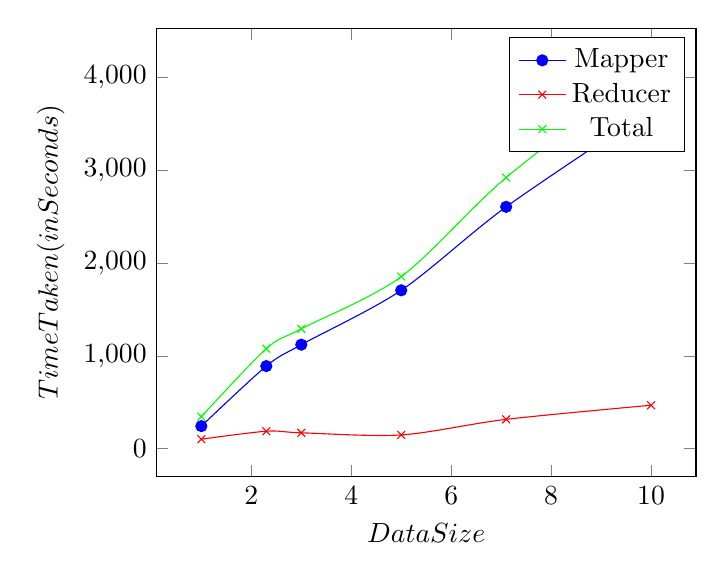
\begin{tikzpicture}
    \begin{axis}[
        xlabel=$DataSize$,
        ylabel=$TimeTaken(inSeconds)$]
    \addplot[smooth,mark=*,blue] plot coordinates {
        (10,3662)
        (7.1,2607)
        (5,1707)
        (3, 1121)
        (2.3,890)
        (1.0, 243)
    };
    \addlegendentry{Mapper}

    \addplot[smooth,color=red,mark=x]
        plot coordinates {
            (10,468)
            (7.1,316)
            (5,148)
            (3,171)            
            (2.3,188)
            (1.0,102)
        };
    \addlegendentry{Reducer}
    
    \addplot[smooth,color=green,mark=x]
        plot coordinates {
            (10,4130)
            (7.1,2923)
            (5, 1855)
            (3,1292)            
            (2.3,1078)
            (1.0,345)
        };
    \addlegendentry{Total}    
    
    \end{axis}
    \end{tikzpicture}